\documentclass[11pt,a4paper]{article}

\usepackage[utf8]{inputenc}
\usepackage[T1]{fontenc}
\usepackage{lmodern}
\usepackage{geometry}
\usepackage{setspace}
\usepackage{graphicx}
\usepackage{booktabs}
\usepackage{longtable}
\usepackage{tabularx}
\usepackage{array}
\usepackage{amsmath}
\usepackage{amssymb}
\usepackage{natbib}
\usepackage{hyperref}
\usepackage{xcolor}
\usepackage{caption}
\usepackage{subcaption}
\usepackage{float}
\usepackage{placeins}

\geometry{margin=2.4cm}
\onehalfspacing
\hypersetup{
  colorlinks=true,
  linkcolor=blue!50!black,
  citecolor=blue!50!black,
  urlcolor=blue!50!black
}
\captionsetup{font=small,labelfont=bf}

\title{Sensitivity Analysis in Hierarchical Parameter Spaces for an Agro-Ecological Model: From Pedoclimatic Dominance to Technical Thresholds in MAELIA}

\author{
Benjamin PIANET\thanks{Main author. Université de Lille, France. Corresponding author: \texttt{benjamin.pianet@etu.univ-lille.fr}.}
\and Paul Saves\thanks{Secondary author. IRIT, Université Toulouse Capitole, Toulouse, France.}
\and Benoît Gaudou\thanks{Secondary author. IRIT, Université Toulouse Capitole, Toulouse, France.}
\and Baptiste Lesquoy\thanks{Secondary author. Affiliation to be completed.}
}

\date{Draft version -- \today}

\begin{document}
\maketitle

\begin{abstract}
Agro-ecological simulation models are increasingly used to explore the long-term consequences of technical operations, pedoclimatic heterogeneity and management choices. Their systematic exploration remains difficult because the parameter space is high-dimensional, partly categorical, and often hierarchical: some parameters are only meaningful when upstream choices activate the corresponding technical operation. This paper presents a sensitivity-analysis workflow for MAELIA, an agro-ecological simulation model, with a focus on hierarchical agricultural-operation parameters. We first show that, on the initial spatially heterogeneous terrain, climate and soil type dominate the variability of the outputs, making the direct interpretation of technical parameters difficult. We then introduce a controlled terrain, \texttt{terrainSA}, built by cloning the same field parcel, \texttt{beauce\_5\_1}, in order to hold soil and climate constant while preserving a large batch of simulations. On this controlled design, we compare surrogate models and retain ExtraTrees as the best metamodel for nitrogen leaching, organic-carbon variation and yield, with test $Q^2$ values of 0.863, 0.991 and 0.959, respectively. The metamodel is used to estimate global indices, including total Sobol indices and Shapley effects, while descriptive ANOVA/Kruskal analyses provide direct evidence on dominant factors and interactions. Finally, interpretable regression trees are trained to identify local threshold regimes. The results show that sowing date and harvest timing dominate nitrogen leaching, whereas fertilization structure drives yield and organic-carbon variation. The proposed workflow illustrates how sensitivity analysis can be adapted to hierarchical parameter spaces by separating environmental heterogeneity, global ranking and local threshold identification.
\end{abstract}

\noindent\textbf{Keywords:} sensitivity analysis; hierarchical parameter space; surrogate modelling; agent-based simulation; agro-ecological modelling; MAELIA; Sobol indices; Shapley effects; decision trees.

\section{Introduction}

Agro-ecological models are expected to support reasoning about cropping systems, technical operations and environmental impacts under heterogeneous spatial and climatic conditions. They are useful precisely because they can combine many processes that are difficult to isolate experimentally: crop development, soil response, climate forcing, plot geometry, farm management and calendars of technical operations. This modelling capacity comes with a methodological cost. When the number of input factors is large, and when some inputs are only meaningful conditionally on previous choices, the model cannot be explored by simple one-factor-at-a-time experiments without losing interactions or creating incoherent scenarios.

This difficulty is especially visible in agent-based and spatially explicit models. The literature on agent-based model exploration has repeatedly emphasized the need to move beyond single trajectories and nominal scenarios toward systematic sensitivity analysis \citep{borgonovo2022protocol,tenbroeke2016which,thiele2014cookbook}. However, classical global sensitivity-analysis methods were mostly developed for rectangular numerical input spaces, whereas many simulation models contain mixed, constrained and conditional parameters. In agricultural simulations, for example, the date and dose of a second fertilization event are not meaningful if the crop itinerary includes no second fertilization. Likewise, a soil-preparation option may activate additional timing and type parameters. The resulting parameter space is hierarchical: upstream discrete decisions activate downstream continuous and categorical variables.

The present work addresses this problem in the context of MAELIA, an agro-ecological simulation model. The initial objective was practical: identify which parameters should be prioritized for future sensitivity analysis of technical operations. The first attempt, performed on a heterogeneous terrain, revealed a strong dominance of soil and climate. This is scientifically meaningful but methodologically limiting. It means that a sensitivity analysis performed directly on the spatially heterogeneous terrain is mostly a sensitivity analysis of pedoclimatic context, not of agronomic operations. Therefore, a second controlled design was built: \texttt{terrainSA}, a terrain composed of repeated clones of the same field parcel. The cloned parcels share the same geometry, soil type and weather polygon, so that variation among simulations comes primarily from the sampled technical parameters.

This paper proposes a three-stage workflow. First, we use the initial terrain to diagnose the dominance of pedoclimatic variation. Second, we use \texttt{terrainSA} to train and validate metamodels, then compute sensitivity indicators in the controlled technical parameter space. Third, we use decision-tree regressors to identify local threshold regimes that can be interpreted as agronomic tipping points. This strategy is aligned with recommendations in the ABM sensitivity-analysis literature: simple descriptive and screening tools are used to understand the response structure, while surrogate models are introduced when the simulator is too expensive for direct Monte Carlo exploration \citep{thiele2014cookbook,tenbroeke2016which,saves2026mabs}.

The contribution of the paper is threefold. First, it demonstrates why environmental heterogeneity must be diagnosed before interpreting technical sensitivity. Second, it provides a practical way to explore a hierarchical agricultural parameter space while preserving constraints between operations. Third, it combines global sensitivity indices and local threshold extraction to obtain both variable ranking and interpretable regimes.

\section{Background and methodological positioning}

\subsection{Sensitivity analysis for complex simulation models}

Sensitivity analysis asks how variation in model inputs propagates to variation in model outputs. In complex simulation models, this is not only a numerical exercise. It is also a way to understand mechanisms, assess robustness, and decide where calibration or further data collection should be focused. \citet{borgonovo2022protocol} propose a protocol for agent-based models that starts with the choice of outputs, clarifies the objective of the analysis, selects the model elements to vary, and then chooses an experimental design and visualizations. A key message is that sensitivity analysis should not be restricted to scalar numerical parameters: assumptions, procedures and behavioural rules may also be varied, often as categorical factors.

\citet{tenbroeke2016which} compare several sensitivity-analysis strategies for agent-based models and emphasize that each method answers a different question. Extended one-factor-at-a-time approaches can reveal nonlinearities and tipping points, while variance-based methods quantify global contributions and interactions. Their recommendation is not to seek a single universal method, but to combine exploratory and global methods according to the modelling objective. \citet{thiele2014cookbook} reach a similar practical conclusion in their cookbook for parameter estimation and sensitivity analysis: begin with simple sampling and screening methods, use global methods when interactions matter, and keep computational cost in mind.

This framing is particularly relevant here. MAELIA is not treated as a simple deterministic function on a small box of continuous inputs. It is a structured agro-ecological simulator whose meaningful input combinations are constrained. A technical itinerary contains hierarchical dependencies: if no fertilization is applied, the number, type, dose and timing of fertilization events are inactive. Therefore, sensitivity analysis must account for both the hierarchy of decisions and the computational cost of simulation.

\subsection{Hierarchical parameter spaces}

A hierarchical parameter space is an input domain in which the availability or meaning of a variable depends on the value of another variable. In the present case, the variable \texttt{n\_ferti} controls the number of fertilization events, and several downstream variables describe the timing, product type and dose of each event. Similar dependencies occur for soil preparation. This structure creates two methodological risks.

First, naive sampling may generate invalid or semantically meaningless configurations. A design point may contain a dose for a third fertilization event even when the corresponding itinerary includes only one fertilization. Second, standard variance-based designs such as Saltelli sampling assume rectangular, independent input dimensions. When these dimensions are unfolded without constraints, hybrid points can violate the model hierarchy. This is a known difficulty for hierarchical and architecture-design spaces, where surrogate modelling and sensitivity analysis must preserve activation rules \citep{saves2026hierarchical}.

In this work, we use a constrained design generated through the existing MAELIA parameterization pipeline. The analysis is then performed on reconstructed agricultural parameters, distinguishing categorical activation variables from continuous timing and dose variables. The key methodological choice is to interpret the resulting inputs as a constrained hierarchical space rather than as independent free variables.

\subsection{Surrogate models and local explanations}

Global sensitivity indices may be computationally expensive when each simulation takes several seconds or minutes. A common solution is to train a surrogate model, or metamodel, on a limited set of simulator evaluations and then use the surrogate for fast exploration \citep{angione2022surrogate,saves2026mabs}. Tree-based models are attractive in this setting because they handle mixed nonlinear responses and interactions without strong parametric assumptions. ExtraTrees, in particular, average many randomized trees and often provide strong predictive performance on tabular data \citep{geurts2006extremely}.

Surrogates also need interpretation. A high predictive score is not sufficient if the objective is scientific understanding. Global sensitivity indices such as Sobol indices \citep{sobol2001global,saltelli2002best} and Shapley effects \citep{shapley1953value,song2016shapley} help quantify contributions, while decision trees provide local threshold rules \citep{breiman1984cart}. This combination mirrors recent multi-stage workflows for agent-based models: coarse screening identifies dominant variables, machine-learning surrogates model nonlinear structure, and explainable tools identify local regimes \citep{saves2026mabs}.

\section{Model outputs and experimental material}

\subsection{Outputs of interest}

The analysis focuses on three outputs extracted from MAELIA simulation logs:

\begin{itemize}
  \item \textbf{Nitrogen leaching} (\texttt{N\_lixi}), a proxy for nitrogen losses and environmental pressure.
  \item \textbf{Organic-carbon variation} (\texttt{dCorg}), a proxy for change in soil organic carbon over the simulation period.
  \item \textbf{Yield} (\texttt{rdt}), the agronomic production output.
\end{itemize}

These outputs represent complementary dimensions of agro-ecological performance. Nitrogen leaching captures an environmental externality, organic carbon captures a soil-quality dimension, and yield captures production. The three outputs may respond differently to sowing dates, harvest dates, fertilization choices and soil-preparation operations. Therefore, sensitivity analysis is performed separately for each output.

\subsection{Initial heterogeneous terrain}

The first analysis used a terrain where several plots differed in soil and climate. This setting reflects the realistic spatial heterogeneity of MAELIA inputs, but it also introduces a strong environmental signal. The resulting figures show that climate zones and soil types structure the distributions of all three outputs. In this setting, the contribution of technical parameters cannot be interpreted independently from pedoclimatic variation.

\begin{figure}[H]
\centering
\begin{subfigure}{0.32\textwidth}
\includegraphics[width=\linewidth]{../figs/rdt_sol_climat.png}
\caption{Yield.}
\end{subfigure}
\hfill
\begin{subfigure}{0.32\textwidth}
\includegraphics[width=\linewidth]{../figs/Nlixi_sol_climat.png}
\caption{Nitrogen leaching.}
\end{subfigure}
\hfill
\begin{subfigure}{0.32\textwidth}
\includegraphics[width=\linewidth]{../figs/Corg_sol_climat.png}
\caption{Organic carbon.}
\end{subfigure}
\caption{Output distributions by soil and climate groups in the initial heterogeneous terrain. The separation between groups shows that pedoclimatic context dominates the first analysis.}
\label{fig:soil-climate}
\end{figure}

A first metamodel trained on these heterogeneous data did not generalize sufficiently well to support a deeper sensitivity analysis. This negative result is important: it confirms that the response surface mixes environmental heterogeneity and technical variation in a way that is difficult to approximate directly. Consequently, the second experimental design was built to control the environmental component.

\subsection{Controlled \texttt{terrainSA} design}

The controlled terrain, \texttt{terrainSA}, is based on repeated clones of the parcel \texttt{beauce\_5\_1}. The clones share the same field geometry, soil properties and weather polygon. The objective is not to represent a realistic landscape, but to isolate the technical itinerary signal while preserving enough simulated observations for sensitivity analysis. This design transforms the question from ``which soil-climate contexts dominate the outputs?'' to ``which agricultural operations matter once soil and climate are fixed?''

The dataset used for the metamodel contains 10,000 observations. It reconstructs 26 agricultural parameters, including activation variables, operation counts, operation types, dates, delays and doses. Fourteen parameters are treated as categorical, while the remaining timing and dose variables are treated as continuous. The hierarchical structure of these variables is maintained by the sampling and simulation pipeline.

\section{Methods}

\subsection{Direct ANOVA/Kruskal screening}

The first controlled analysis is descriptive. For each output and parameter, continuous variables are discretized into quantile groups and categorical variables are used as factors. Depending on normality and homoscedasticity diagnostics, either an ANOVA-like comparison or a Kruskal test is used. The reported quantity is an empirical $R^2$:
\begin{equation}
R^2_j = \frac{SS_{\mathrm{between},j}}{SS_{\mathrm{total}}},
\end{equation}
where $SS_{\mathrm{between},j}$ is the between-group sum of squares induced by parameter $j$. This quantity should be read as descriptive variance explained by grouped parameter values, not as a causal estimator.

Two-factor analyses are then computed to separate additive and interaction effects. For a pair $(A,B)$, the interaction contribution is measured as the gain in $R^2$ between a saturated grouped model and an additive grouped model. This provides a matrix of pairwise interaction signals for each output.

\subsection{Metamodel comparison and global indices}

The second analysis trains surrogate models to approximate each output from the agricultural parameters. ExtraTrees, XGBoost and Gaussian-process regressors are compared. The retained model is selected by test $Q^2$, defined as the coefficient of determination on a held-out test set. ExtraTrees is retained for all three outputs.

The selected surrogate is used for global sensitivity analysis. Sobol first-order and total-order indices are estimated by Monte Carlo sampling over the reconstructed parameter domain. First-order indices measure direct contributions, while total-order indices include interactions. Shapley effects are also estimated to obtain an allocation of explained variance that accounts for all coalitions of variables. Since the original design is not a pure Saltelli design, these global indices are interpreted as metamodel-based sensitivity summaries rather than direct simulator-based estimators.

\subsection{Decision-tree threshold analysis}

The final analysis trains constrained decision-tree regressors for each output. The objective is interpretability rather than maximum prediction. The trees are tuned by cross-validation over maximum depth, minimum leaf size and pruning parameter. Each split defines a local threshold or categorical rule. Leaf summaries provide mean output values within local regimes.

A complementary residual analysis is also performed. A simple additive model is fitted first, then a decision tree is trained on its residuals. This identifies local nonlinear structure remaining after additive effects. Such a procedure follows the logic of using simple methods for screening and tree-based tools for identifying threshold regimes, as recommended for complex ABM exploration \citep{tenbroeke2016which,saves2026mabs}.

\section{Results}

\subsection{Pedoclimatic dominance in the initial analysis}

The first result is that soil and climate dominate the initial sensitivity analysis. The grouped output figures in Figure~\ref{fig:soil-climate} show strong separation by environmental context. ANOVA and PRCC visualizations support the same conclusion: before any technical interpretation, the spatial heterogeneity of soil and weather explains a major part of output variability.

\begin{figure}[H]
\centering
\begin{subfigure}{0.48\textwidth}
\includegraphics[width=\linewidth]{../figs/ANOVA.png}
\caption{ANOVA-style screening.}
\end{subfigure}
\hfill
\begin{subfigure}{0.48\textwidth}
\includegraphics[width=\linewidth]{../figs/PRCC.png}
\caption{PRCC screening.}
\end{subfigure}
\caption{Initial screening on the heterogeneous terrain. The analysis is dominated by the environmental structure of the terrain.}
\label{fig:first-screening}
\end{figure}

This finding motivated the controlled \texttt{terrainSA} experiment. Without this control, a technical parameter might appear unimportant simply because pedoclimatic variation is larger, or conversely appear important because it is confounded with environmental grouping. The separation between the two stages is therefore not only computational; it is required for interpretation.

\subsection{Metamodel performance on \texttt{terrainSA}}

On the controlled dataset, ExtraTrees outperformed the other candidate models and generalized well on held-out observations. Table~\ref{tab:metamodel} reports the retained metamodel and the main predictive metrics.

\begin{table}[H]
\centering
\caption{Performance of the retained metamodel on \texttt{terrainSA}.}
\label{tab:metamodel}
\begin{tabular}{lrrrr}
\toprule
Output & Model & Test $Q^2$ & MAE & RMSE \\
\midrule
\texttt{N\_lixi} & ExtraTrees & 0.863 & 0.196 & 0.282 \\
\texttt{dCorg} & ExtraTrees & 0.991 & 5.207 & 8.953 \\
\texttt{rdt} & ExtraTrees & 0.959 & 0.045 & 0.071 \\
\bottomrule
\end{tabular}
\end{table}

The lower score for \texttt{N\_lixi} suggests a more complex or noisier response surface for leaching, but the predictive quality remains sufficient for exploratory global indices. The very high scores for \texttt{dCorg} and \texttt{rdt} indicate that the technical parameter space contains a strong and learnable signal once soil and climate are fixed.

\subsection{Direct factor screening}

The one-factor analysis identifies different dominant factors for each output. Table~\ref{tab:anova-one} summarizes the leading descriptive $R^2$ values.

\begin{table}[H]
\centering
\caption{Leading one-factor descriptive $R^2$ values on \texttt{terrainSA}.}
\label{tab:anova-one}
\begin{tabular}{lll}
\toprule
Output & Dominant parameters & Interpretation \\
\midrule
\texttt{N\_lixi} & \texttt{Jour\_Semis} ($R^2=0.341$), \texttt{Jours\_op\_recolte} ($0.082$) & calendar effects dominate leaching \\
\texttt{dCorg} & \texttt{n\_ferti} ($0.432$), \texttt{Jours\_semis\_F1} ($0.388$) & fertilization structure drives carbon response \\
\texttt{rdt} & \texttt{n\_ferti} ($0.568$), \texttt{Jours\_semis\_F1} ($0.344$) & fertilization dominates yield \\
\bottomrule
\end{tabular}
\end{table}

\begin{figure}[H]
\centering
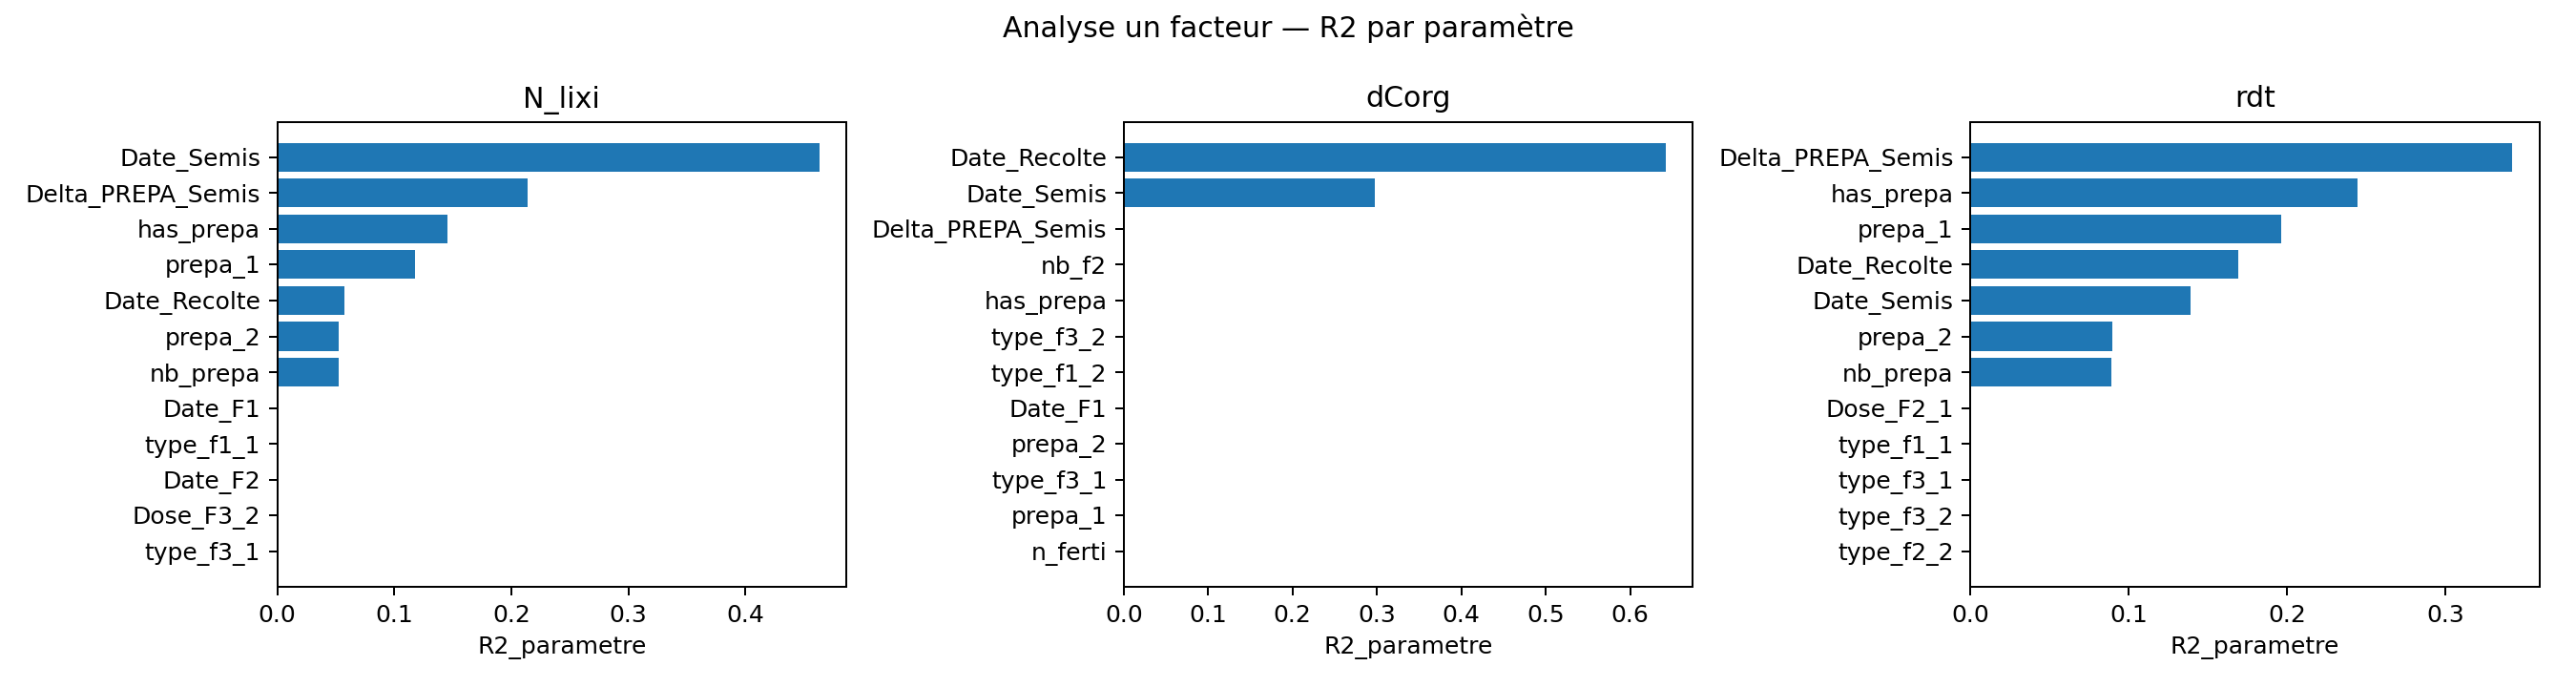
\includegraphics[width=0.9\textwidth]{../analysis/terrainSA_results/anova_1facteur_top.png}
\caption{Top one-factor ANOVA/Kruskal effects by output on \texttt{terrainSA}.}
\label{fig:anova-one}
\end{figure}

The result is consistent across methods. Nitrogen leaching is mainly calendar-driven, especially by sowing date and harvest timing. Organic-carbon variation and yield are more strongly driven by the structure of fertilization: the number of fertilization events, their timing and dose distribution.

\subsection{Pairwise interactions}

Pairwise interaction matrices reveal that interactions are present but generally smaller than the leading main effects. The strongest interaction signals combine dates and fertilization variables. For \texttt{N\_lixi}, interactions involving sowing-to-fertilization delay and harvest timing are visible. For \texttt{dCorg} and \texttt{rdt}, interactions involving \texttt{n\_ferti}, \texttt{Jours\_semis\_F1}, \texttt{Dose\_F1\_1} and harvest timing are more prominent.

\begin{figure}[H]
\centering
\begin{subfigure}{0.32\textwidth}
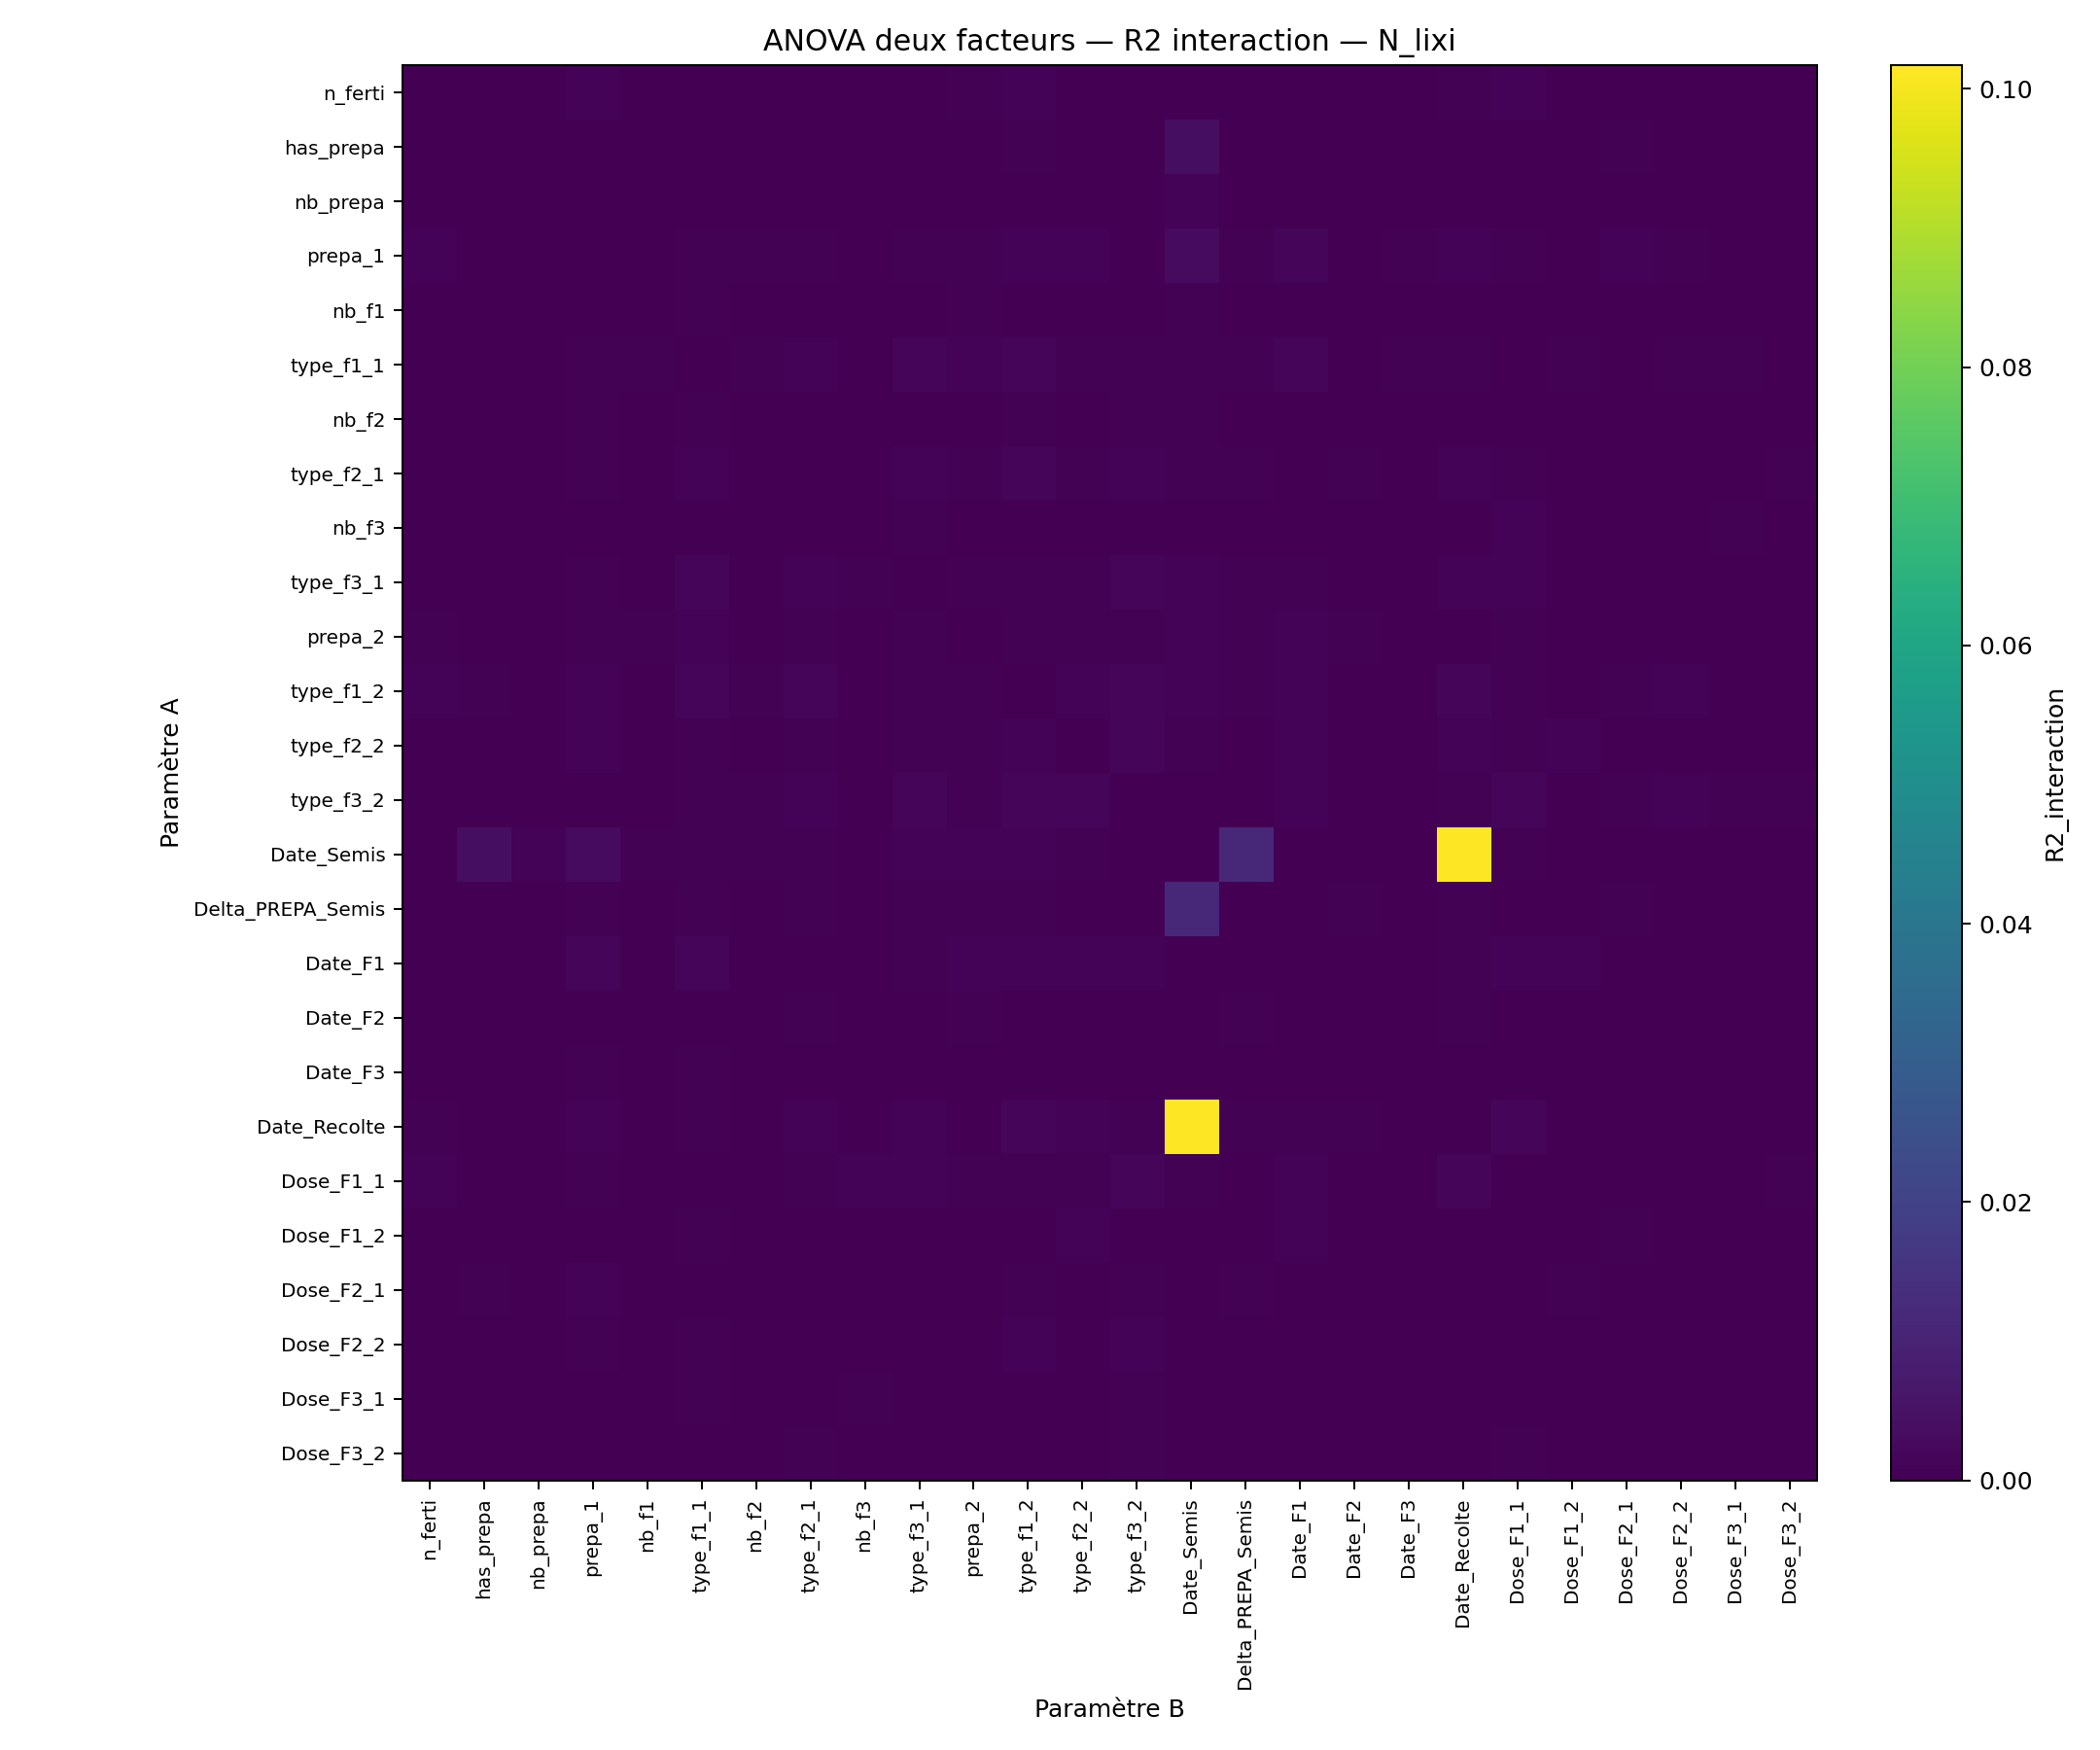
\includegraphics[width=\linewidth]{../analysis/terrainSA_results/heatmap_anova_2facteurs_R2_interaction_N_lixi.png}
\caption{\texttt{N\_lixi}.}
\end{subfigure}
\hfill
\begin{subfigure}{0.32\textwidth}
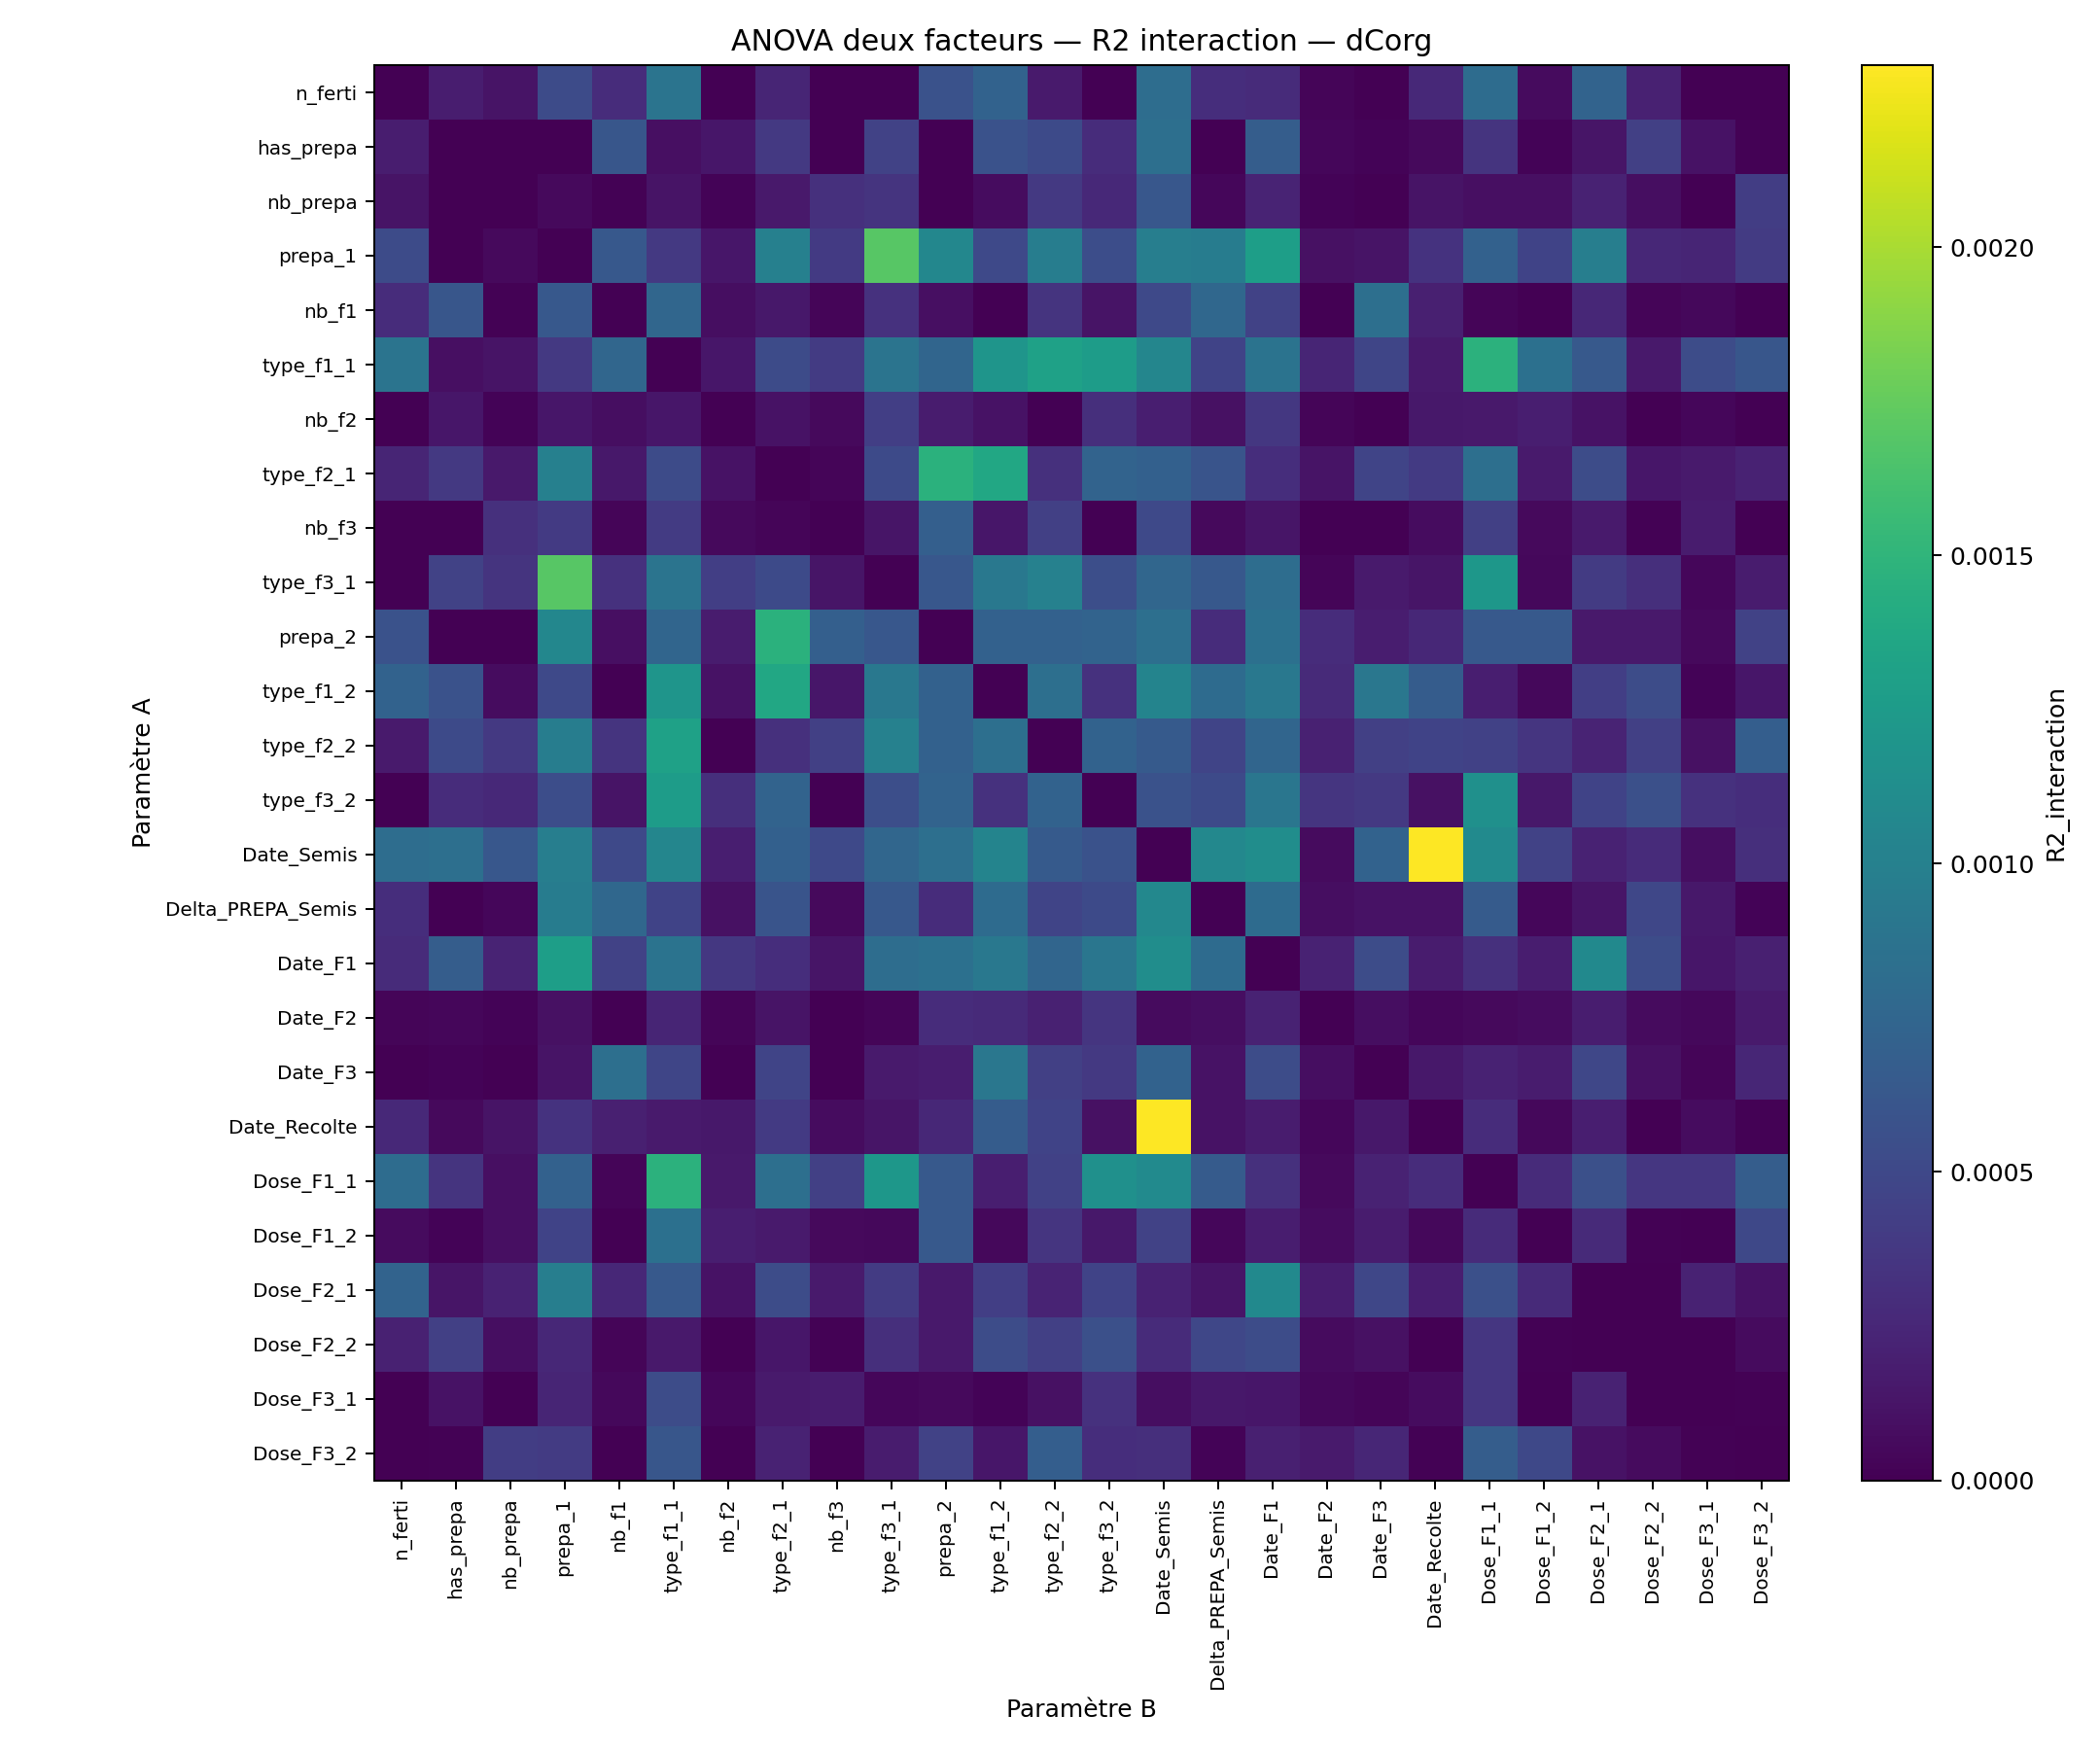
\includegraphics[width=\linewidth]{../analysis/terrainSA_results/heatmap_anova_2facteurs_R2_interaction_dCorg.png}
\caption{\texttt{dCorg}.}
\end{subfigure}
\hfill
\begin{subfigure}{0.32\textwidth}
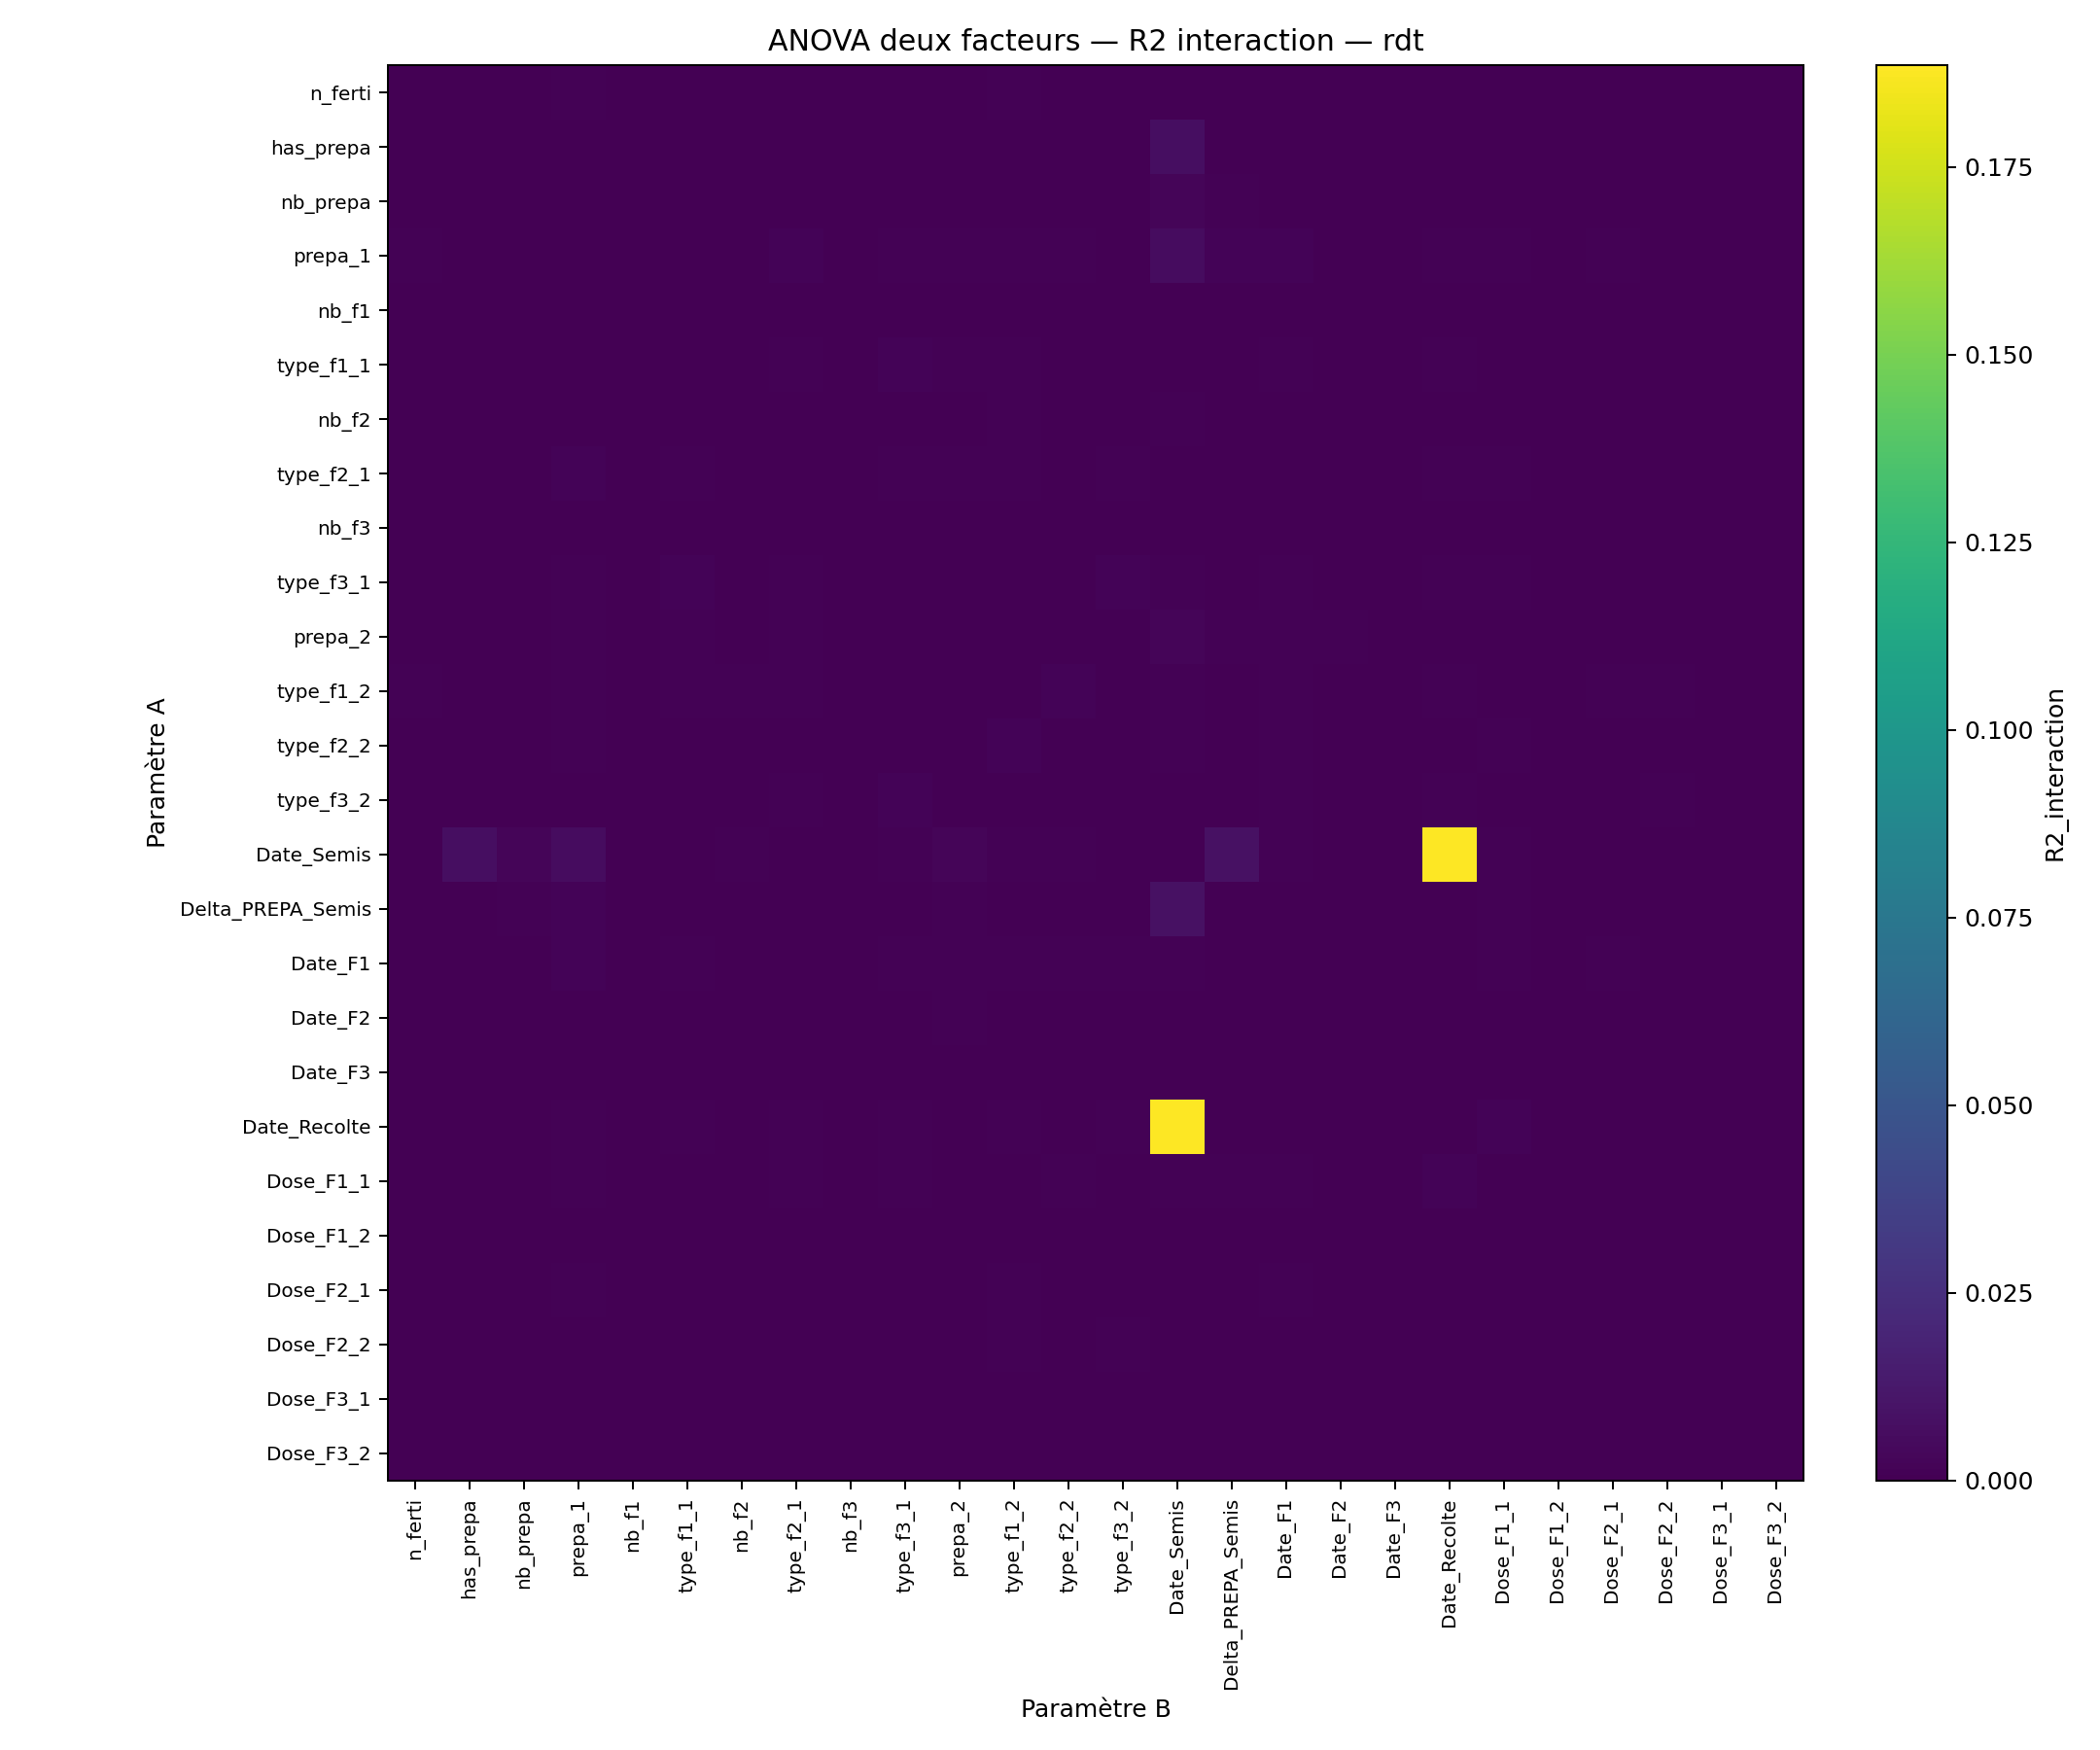
\includegraphics[width=\linewidth]{../analysis/terrainSA_results/heatmap_anova_2facteurs_R2_interaction_rdt.png}
\caption{\texttt{rdt}.}
\end{subfigure}
\caption{Pairwise interaction $R^2$ heatmaps. Only the interaction component is shown, excluding additive effects.}
\label{fig:interaction-heatmaps}
\end{figure}

These matrices should be read as a guide to local phenomena, not as a complete decomposition of the hierarchical space. They identify combinations worth further examination, especially when a calendar variable modifies the effect of fertilization.

\subsection{Sobol and Shapley effects through the metamodel}

The Sobol total-order indices and Shapley effects provide a global ranking that is broadly consistent with the direct analysis. Figure~\ref{fig:sobol-shapley} shows the main summaries.

\begin{figure}[H]
\centering
\begin{subfigure}{0.48\textwidth}
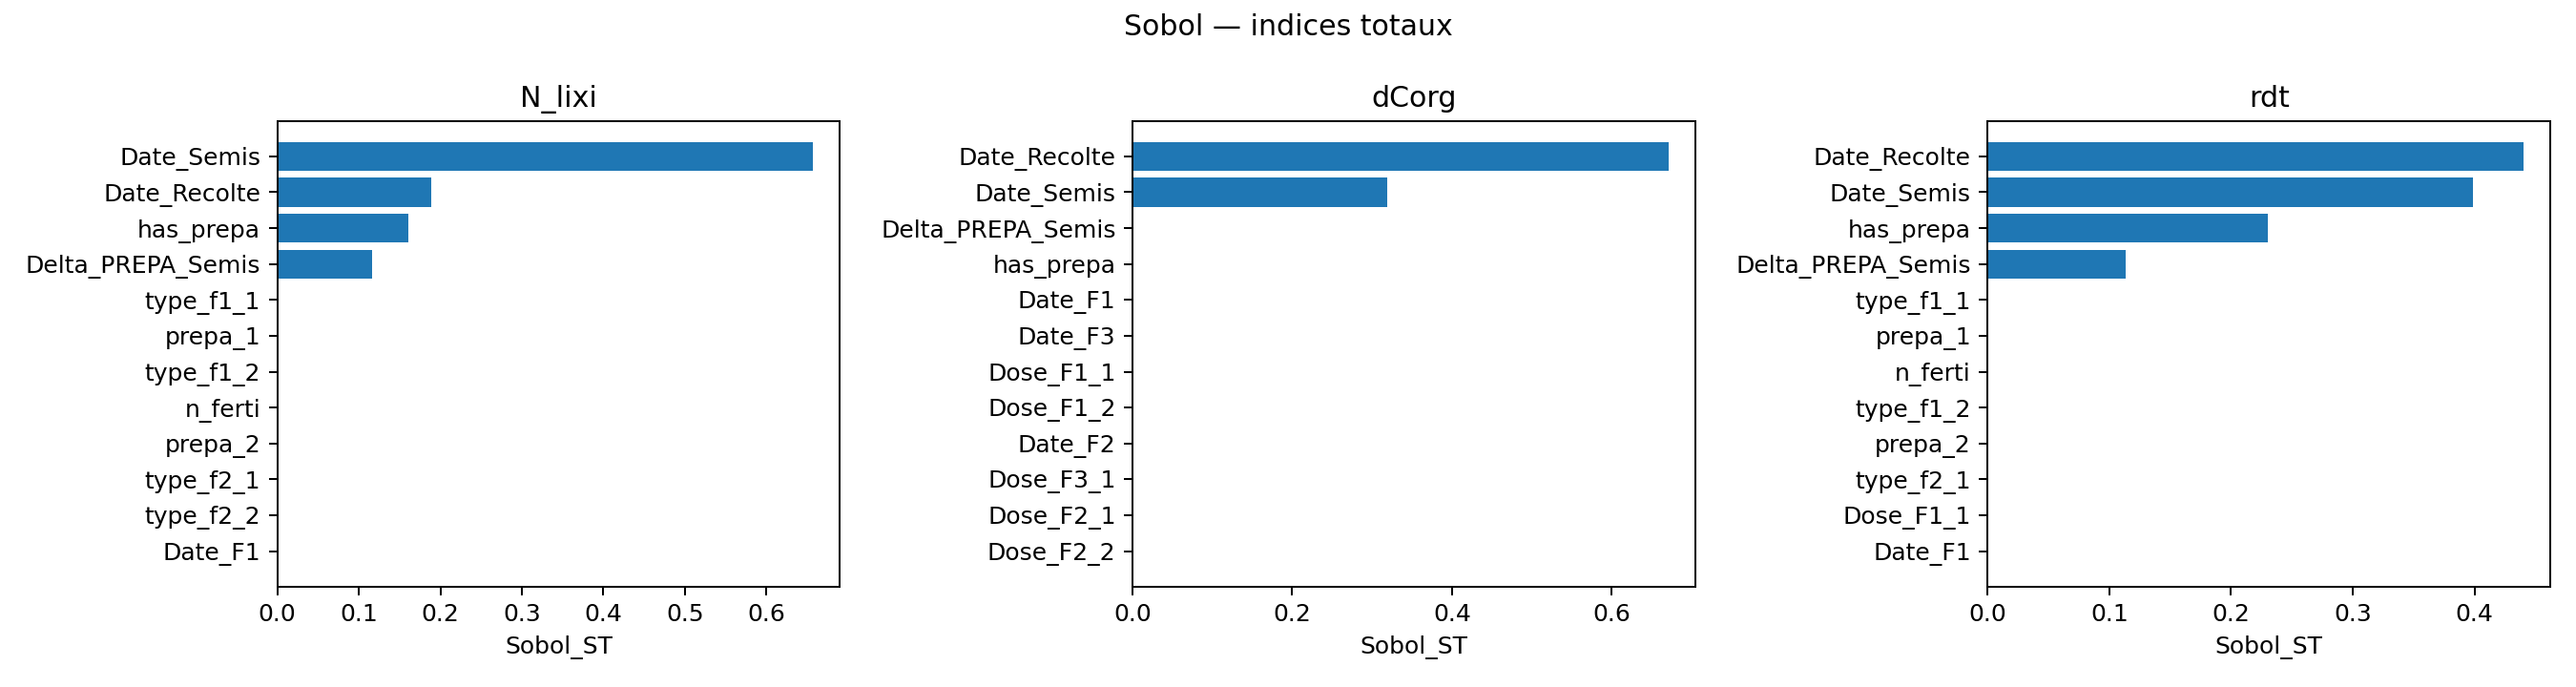
\includegraphics[width=\linewidth]{../analysis/terrainSA_results/sobol_total_top.png}
\caption{Sobol total-order indices.}
\end{subfigure}
\hfill
\begin{subfigure}{0.48\textwidth}
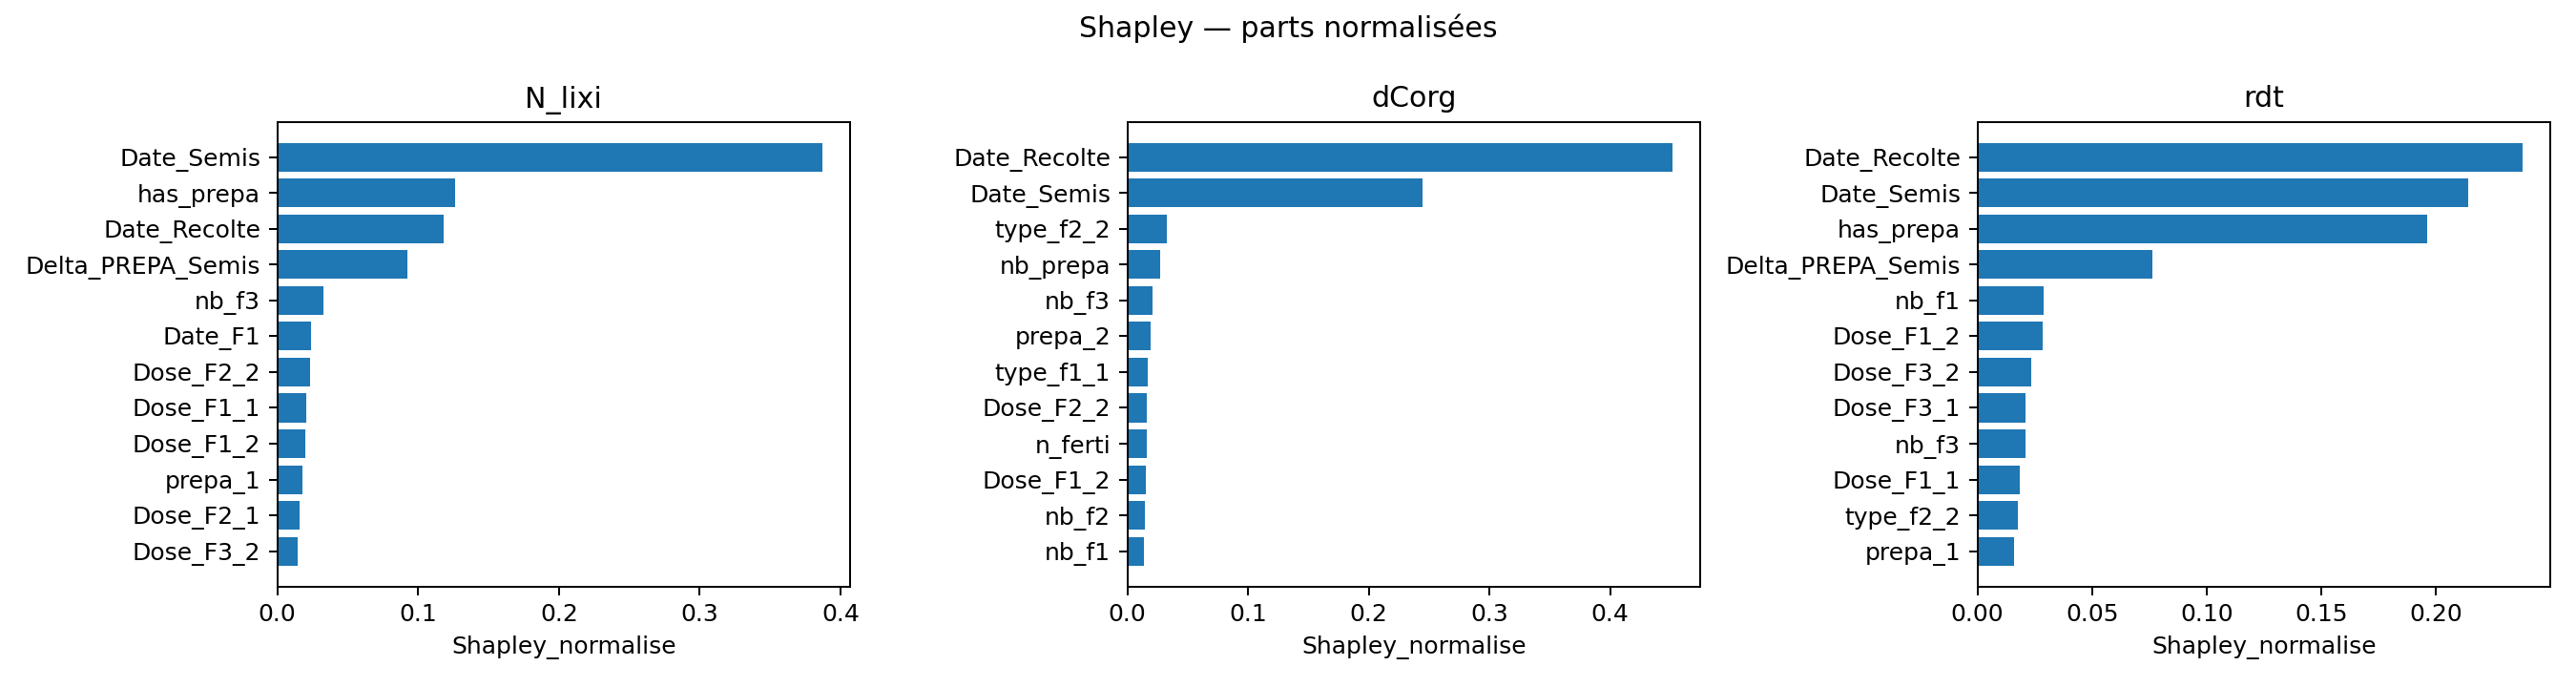
\includegraphics[width=\linewidth]{../analysis/terrainSA_results/shapley_top.png}
\caption{Shapley effects.}
\end{subfigure}
\caption{Global sensitivity summaries estimated from the retained ExtraTrees metamodel.}
\label{fig:sobol-shapley}
\end{figure}

For \texttt{N\_lixi}, \texttt{Jour\_Semis} is dominant. Its Sobol first-order index is 0.590 and its total-order index is 0.519, while its normalized Shapley effect is 0.317. \texttt{Jours\_op\_recolte} is the second major factor, with a total-order index of 0.302 and a Shapley effect of 0.146. Fertilization count and first fertilization timing contribute less individually but remain relevant through interactions.

For \texttt{dCorg}, \texttt{n\_ferti} is the leading variable in both ANOVA and Shapley summaries. The tree and Shapley results indicate that organic-carbon variation responds strongly to whether fertilization is present and how it is scheduled. For \texttt{rdt}, the dominance of \texttt{n\_ferti} is even clearer, followed by \texttt{Jours\_semis\_F1} and dose-related variables.

\subsection{Decision-tree thresholds}

Decision-tree regressors were trained to extract local regimes. Their predictive performance is lower than ExtraTrees, as expected, but remains useful for interpretation (Table~\ref{tab:tree}).

\begin{table}[H]
\centering
\caption{Performance and dominant variables of interpretable regression trees.}
\label{tab:tree}
\begin{tabularx}{\textwidth}{lrlX}
\toprule
Output & Test $Q^2$ & Max depth & Main variables used \\
\midrule
\texttt{N\_lixi} & 0.596 & 5 & \texttt{Jour\_Semis}, \texttt{Jours\_op\_recolte}, \texttt{Jours\_semis\_F1}, \texttt{n\_ferti} \\
\texttt{dCorg} & 0.863 & 5 & \texttt{n\_ferti}, \texttt{Jours\_op\_recolte}, \texttt{Jours\_semis\_F1} \\
\texttt{rdt} & 0.813 & 5 & \texttt{n\_ferti}, \texttt{Jours\_semis\_F1}, \texttt{Jours\_op\_recolte}, \texttt{Jour\_Semis} \\
\bottomrule
\end{tabularx}
\end{table}

\begin{table}[H]
\centering
\caption{Examples of local thresholds extracted from decision trees. Means are the training-set means on both sides of the rule.}
\label{tab:thresholds}
\begin{tabularx}{\textwidth}{llr}
\toprule
Output & Rule & Mean values separated by the rule \\
\midrule
\texttt{N\_lixi} & \texttt{Jour\_Semis} $\leq 284.3$ vs. $>284.3$ & 3.21 vs. 4.09 \\
\texttt{N\_lixi} & \texttt{Jours\_op\_recolte} $\leq 67.34$ vs. $>67.34$ & 2.66 vs. 3.82 \\
\texttt{dCorg} & \texttt{n\_ferti} $\neq 0$ vs. $=0$ & -251 vs. -120 \\
\texttt{dCorg} & \texttt{Jours\_op\_recolte} $\leq 97.76$ vs. $>97.76$ & -196 vs. -303 \\
\texttt{rdt} & \texttt{n\_ferti} $\neq 0$ vs. $=0$ & 4.27 vs. 3.67 \\
\texttt{rdt} & \texttt{Jours\_semis\_F1} $\leq 169.2$ vs. $>169.2$ & 3.81 vs. 4.31 \\
\bottomrule
\end{tabularx}
\end{table}

\begin{figure}[H]
\centering
\begin{subfigure}{0.32\textwidth}

\includegraphics[width=\linewidth]{../analysis/decision_tree_thresholds/decision_tree_N_lixi.png}
\caption{\texttt{N\_lixi}.}
\end{subfigure}
\hfill
\begin{subfigure}{0.32\textwidth}

\includegraphics[width=\linewidth]{../analysis/decision_tree_thresholds/decision_tree_dCorg.png}
\caption{\texttt{dCorg}.}
\end{subfigure}
\hfill
\begin{subfigure}{0.32\textwidth}

\includegraphics[width=\linewidth]{../analysis/decision_tree_thresholds/decision_tree_rdt.png}
\caption{\texttt{rdt}.}
\end{subfigure}
\caption{Regression trees used to identify threshold regimes. The trees are intentionally constrained for interpretability.}
\label{fig:trees}
\end{figure}

For nitrogen leaching, the first global split is a sowing-date threshold around 284 days. Later sowing is associated with higher mean leaching in the tree. Harvest timing then defines local regimes, with thresholds around 67, 124 and 175 days depending on the branch. This suggests that leaching response is not only a matter of fertilizer quantity, but of the calendar alignment between sowing, fertilization and harvest.

For organic-carbon variation, the strongest split is categorical: whether fertilization is absent. Regimes without fertilization are less negative on average for \texttt{dCorg}. Fertilized regimes combined with later harvest and specific fertilization delays produce the most negative carbon changes. This does not imply that fertilization is undesirable in general; it indicates that, in the simulated technical space and time horizon, fertilization structure is a dominant marker of carbon-response regimes.

For yield, the first split is also \texttt{n\_ferti}. Absence of fertilization lowers yield, while fertilized regimes are further separated by first-fertilization timing, harvest timing and sowing date. The best-yield leaves combine fertilization with favorable calendar thresholds.

\begin{figure}[H]
\centering
\begin{subfigure}{0.32\textwidth}
\includegraphics[width=\linewidth]{../analysis/decision_tree_thresholds/decision_tree_importance_N_lixi.png}
\caption{\texttt{N\_lixi}.}
\end{subfigure}
\hfill
\begin{subfigure}{0.32\textwidth}
\includegraphics[width=\linewidth]{../analysis/decision_tree_thresholds/decision_tree_importance_dCorg.png}
\caption{\texttt{dCorg}.}
\end{subfigure}
\hfill
\begin{subfigure}{0.32\textwidth}
\includegraphics[width=\linewidth]{../analysis/decision_tree_thresholds/decision_tree_importance_rdt.png}
\caption{\texttt{rdt}.}
\end{subfigure}
\caption{Feature importances aggregated by original agricultural parameter in the interpretable trees.}
\label{fig:tree-importance}
\end{figure}

Residual trees reveal remaining nonlinear structure after an additive model. The residual-tree $Q^2$ is 0.172 for \texttt{N\_lixi}, 0.591 for \texttt{dCorg} and 0.298 for \texttt{rdt}. This indicates that carbon variation retains the strongest non-additive structure after accounting for additive effects, while nitrogen leaching is more dominated by the direct calendar thresholds already visible in the main tree.

\section{Discussion}

\subsection{Why the controlled terrain matters}

The most important methodological lesson is that sensitivity analysis cannot be separated from the experimental support on which it is performed. On the initial terrain, soil and climate dominate. This is not a failure of sensitivity analysis; it is a correct diagnosis of the model response under spatial heterogeneity. However, it answers a different question from the one asked here. If the objective is to understand technical operations, pedoclimatic variation must either be modelled explicitly as a major factor or controlled.

The \texttt{terrainSA} design implements this control by cloning a single parcel. This is not meant to replace realistic spatial simulations. Instead, it is a local experimental device: it holds environmental conditions fixed so that agricultural operations can be compared. The distinction between realistic heterogeneity and controlled sensitivity is essential for agro-ecological model exploration.

\subsection{Hierarchical spaces and valid scenarios}

The agricultural parameter space is not a simple product of independent intervals. It contains activation rules. Ignoring these rules would create invalid hybrid points and could distort Sobol or Shapley estimates. The current workflow mitigates this problem by relying on a constrained design and by interpreting categorical activation variables explicitly. Still, the metamodel-based global indices should be read as summaries over the sampled constrained distribution, not as universal indices over an unconstrained hypercube.

This point is important for future work. A fully rigorous variance-based analysis in a hierarchical space requires sampling schemes that preserve activation constraints by construction. Recent work on hierarchical design spaces and surrogate-based architecture design provides a useful methodological direction \citep{saves2026hierarchical}. For MAELIA, this would mean generating pick-freeze or Shapley coalitions directly inside the feasible technical-itinerary space.

\subsection{Global ranking and local thresholds}

The workflow intentionally combines global and local tools. ANOVA/Kruskal and Sobol/Shapley summaries answer the question ``which variables matter overall?'' Decision trees answer a different question: ``where does the response change regime?'' Both are needed. For example, \texttt{Jour\_Semis} is globally important for nitrogen leaching, but the decision tree adds a threshold around day 284 and shows that harvest timing matters within specific branches. Similarly, \texttt{n\_ferti} dominates yield and carbon variation, but its effect is modulated by delays and operation timing.

The threshold results should not be interpreted as agronomic recommendations yet. They are model-based hypotheses. Their value is to identify zones of the parameter space where more detailed simulation, expert discussion or targeted experiments should be performed.

\subsection{Limitations}

Several limitations remain. First, \texttt{terrainSA} deliberately removes soil and climate variation. It is therefore a local analysis around one parcel context. The conclusions should not be generalized to all soils or climates without repeating the controlled design across representative environmental contexts. Second, the metamodel is trained on simulated data and inherits both the strengths and limitations of MAELIA. Third, the global Sobol and Shapley indices are estimated through a surrogate and over a constrained sampled design, not directly through a classical Saltelli design. Fourth, decision-tree thresholds depend on the sampled domain and the tree regularization parameters.

Despite these limitations, the staged workflow makes the interpretation more robust. It avoids mixing environmental dominance and technical effects, validates the surrogate before using it for global sensitivity analysis, and complements global rankings with interpretable threshold regimes.

\section{Conclusion}

This paper presented a sensitivity-analysis workflow for MAELIA in a hierarchical agricultural parameter space. The first stage showed that, when soil and climate vary, pedoclimatic context dominates the outputs. The second stage introduced \texttt{terrainSA}, a controlled cloned-parcel design that isolates technical operations. On this dataset, ExtraTrees provided accurate metamodels for nitrogen leaching, organic-carbon variation and yield. Global sensitivity summaries showed that sowing date and harvest timing dominate nitrogen leaching, while fertilization structure dominates yield and carbon variation. The third stage used decision-tree regressors to identify local thresholds, including a sowing-date threshold around day 284 for leaching and strong categorical regimes around the presence or absence of fertilization for yield and carbon.

The main message is methodological. In agro-ecological simulations with hierarchical parameters, sensitivity analysis should not be applied as a single black-box procedure. It should first diagnose environmental dominance, then construct a feasible controlled design, then combine surrogate-based global indices with local threshold tools. This staged approach provides a clearer path from complex simulation logs to interpretable agronomic hypotheses.

\section*{Data and code availability}

The notebooks and generated figures used in this draft are stored in the repository containing the MAELIA sensitivity-analysis workflow. The main analysis notebooks are \texttt{analysis/Analyse\_terrainSA.ipynb} and \texttt{analysis/Analyse\_seuils\_decision\_tree.ipynb}. The controlled simulation notebook is \texttt{simulations/batch\_simulations\_smt\_terrainSA.ipynb}.

\section*{Acknowledgements}

This draft was prepared as part of an internship project on sensitivity analysis for MAELIA. The author thanks the contributors to the MAELIA modelling environment and the methodological discussions around hierarchical spaces and simulation exploration. Funding and institutional acknowledgements should be completed before submission.

\bibliographystyle{plainnat}
\bibliography{references}

\end{document}
